\chapter{METODOLOGI}
\label{sec:chap3_metodologi}

\section*{ }
% Ubah bagian-bagian berikut dengan isi dari desain dan implementasi
Penelitian ini dilaksanakan sesuai dengan desain sistem berikut dengan implementasinya. 
Desain sistem merupakan konsep dari pembuatan dan perancangan infrastruktur dan kemudian diwujudkan dalam 
bentuk blok-blok alur yang harus dikerjakan. Sedangkan untuk bagian implementasi merupakan pelaksanaan teknis 
untuk setiap blok pada desain sistem.

\begin{figure}[h!]
	\begin{center}
	  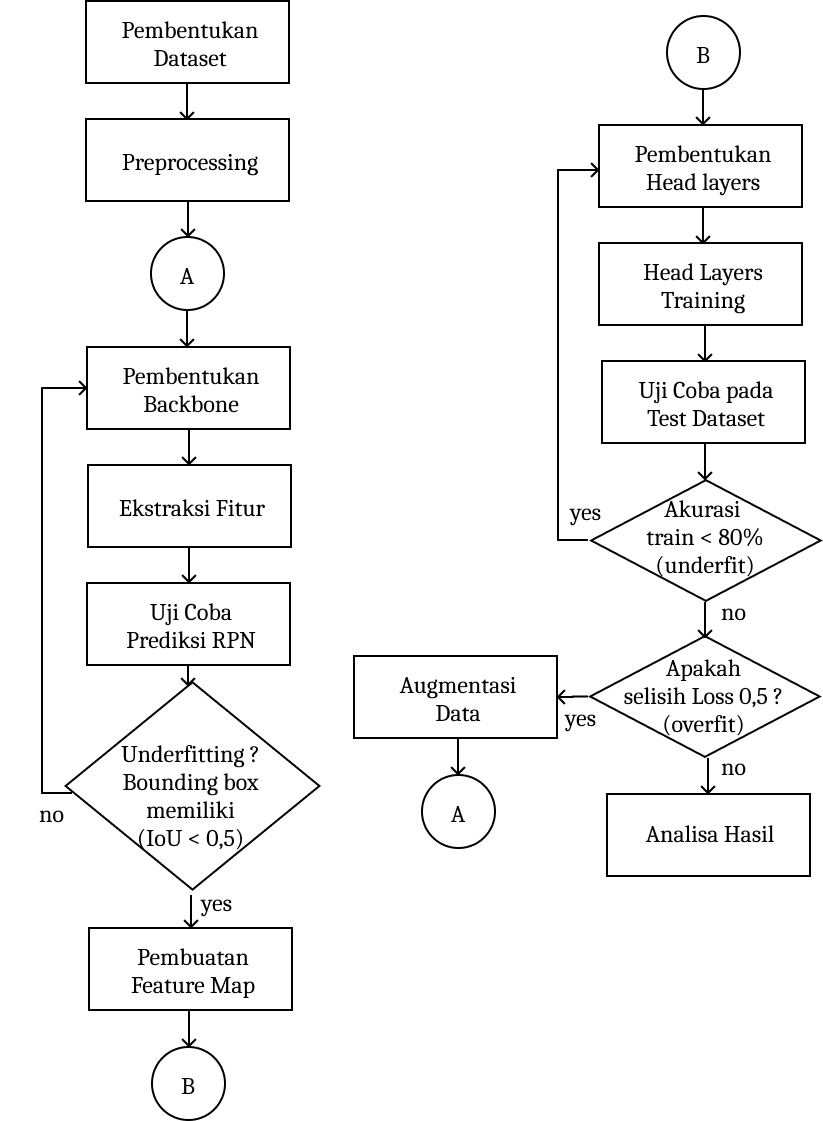
\includegraphics[width= 0.8\linewidth]{bab3/Flow Chart.png}
	  \caption{Bagan Umum Metodologi Penelitian}
	  \label{fig: base_method_1}
	\end{center}
\end{figure}


  Gambar \ref{fig: base_method_1} merupakan bagan yang menunjukkan secara garis besar bagaimana proses pembentukan model
  pada penelitian ini. Penelitian dimulai dengan pembentukan dataset, kemudian dilanjutkan dengan proses \textit{preprocessing}.
  Setelah pembentukan jaringan \textit{backbone}, maka akan dilanjutkan dengan proses ekstraksi fitur menggunakan jaringan
  \textit{backbone} yang telah dibentuk. Kemudian jaringan \textit{backbone} tersebut akan menghasilkan \textit{regional proposal network}
  dan prediksi \textit{bounding box}. Jika model tidak dapat mendeteksi \textit{bounding box} dengan baik dengan kata lain,
  kemiripan \textit{bounding box} yang diprediksi memiliki irisan (IoU) kurang dari 0,5 dengan \textit{bounding box} asli, maka
  jaringan \textit{backbone} perlu dikonfigurasi ulang menggunakan model \textit{backbone} yang berbeda. Kemudian jika model
  \textit{backbone} telah memberikan \textit{bounding box} yang sesuai, maka model \textit{backbone} dapat digunakan untuk
  menghasilkan \textit{feature map}.

  Setelah \textit{feature map} dibentuk, maka \textit{head layers} dibentuk untuk memprediksi kelas dan \textit{bounding box} serta 
  menggenerasi \textit{mask}. Setelah itu lapisan jaringan pada \textit{head} perlu dilatih agar dapat mendeteksi kelas, \textit{bounding box}, Dan
  menggenerasi \textit{mask}. Setelah proses \textit{training} selesai maka model keseluruhan perlu diuji secara keseluruhan dengan
  cara mengujinya dengan dataset tes dan dataset validasi. Setelah itu jika terjadi \textit{underfitting}, maka lapisan \textit{head} perlu
  dimodelkan ulang, namun jika terjadi \textit{overfitting} yaitu dimana loss kumulatif yang terjadi pada \textit{train dataset} memiliki
  nilai 0,5 lebih kecil dibandingkan \textit{test dataset} maka augmentasi data dan penambahan regularisasi diperlukan untuk
  mengurangi selisih \textit{loss} yang terjadi.

  \section{Pembentukan Dataset}
  Pada proses pembentukan dataset, terdapat dua langkah penting yaitu pengumpulan data serta anotasi data. pengumpulan
  data dilakukan dengan mengambil video pada lokasi yang menjadi tempat pengamatan, pada penelitian ini, peneliti 
  menetapkan Pasar Atom yang berada pada alamat Jl. Bunguran No.45, Bongkaran, Kec. Pabean Cantikan, Surabaya. 
  Pasar Atom dinilai sebagai lokasi yang tepat dikarenakan pasar tersebut dinilai modern dan ramai pengunjung.

  \begin{figure}[h!]
    \begin{center}
      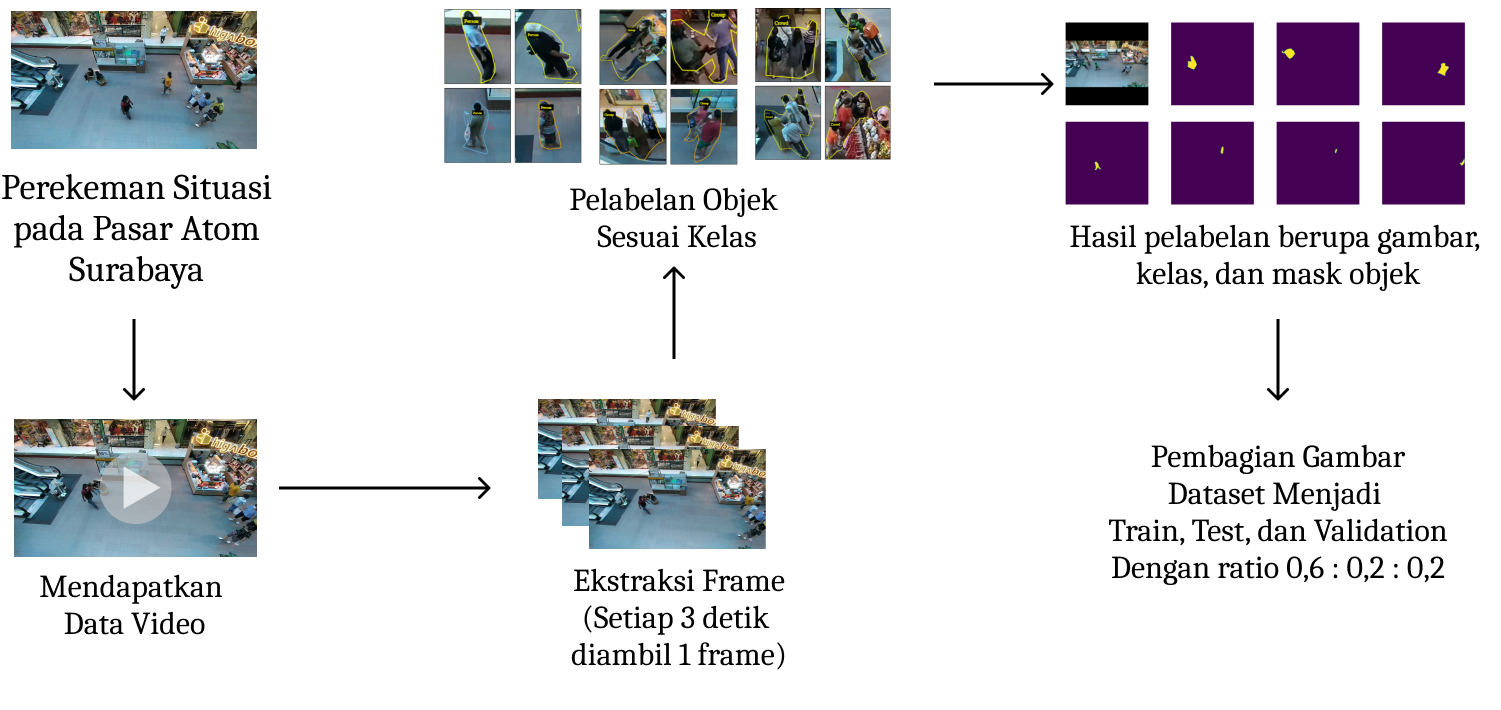
\includegraphics[width= 1.0\linewidth]{bab3/Pembentukan Dataset.png}
      \caption{Alur Pembentukan Dataset}
      \label{fig: base_method}
    \end{center}
  \end{figure}
  
  \subsection{Pengumpulan Data}
  Pada proses pengumpulan data, data mengenai aktivitas pembeli, penjual, dan petugas yang berada pada Pasar Atom
  akan diambil dalam bentuk video. Data tersebut akan diambil di berbagai lokasi pengamatan yang masih berada pada 
  kawasan Pasar Atom. Data video tersebut kemudian akan diubah menjadi gambar dengan cara mengekstrak satu gambar setiap
  tiga \textit{frame} pada video. Beberapa lokasi yang menjadi pengamatan ialah pintu masuk utama Pasar Atom, 
  lantai dua Pasar Atom, dan eskalator utama Pasar Atom. Pengumpulan data dilakukan menggunakan kamera 8 Mega Pixel dimana 
  tinggi kamera adalah 5 meter dan mempunyai sudut 30 derajat terhadap sumbu X. Data yang dikumpulkan merupakan data video
  berukuran 1920 x 1080 px.

  \begin{figure}[h!]
    \begin{center}
      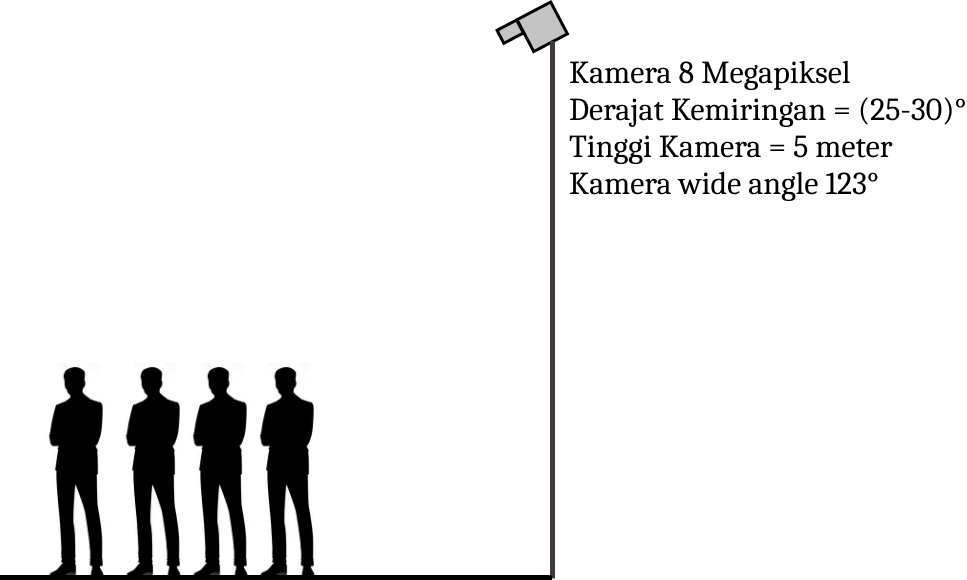
\includegraphics[width= 0.7\linewidth]{bab3/Konfigurasi tinggi kamera.png}
      \caption{Konfigurasi Pengambilan Gambar}
      \label{fig: base_method}
    \end{center}
  \end{figure}
  
  \subsection{Anotasi Data}
  Pada proses ini, data yang telah berupa gambar tersebut akan dianotasi menjadi tiga kelas sebagai berikut :
  
  \begin{itemize}
	  \item \textbf{Kelas \textit{Person}}
	  
	  Kelas \textit{Person} diberikan kepada objek orang yang tidak berada di dekat orang lain dalam jarak radius
	  satu meter.
  
	  \item \textbf{Kelas \textit{Group}}
	  
	  Kelas \textit{Group} diberikan kepada objek kelompok orang yang terdiri dari dua hingga tiga orang dalam
	  radius satu meter.
  
	  \item \textbf{Kelas \textit{Crowd}}
	  
	  Kelas \textit{Crowd} diberikan kepada objek kelompok orang yang terdiri dari empat atau lebih orang dalam
	  radius satu meter.
  \end{itemize}
  
  Proses anotasi dilakukan dengan \textit{software VGG Image Annotator (VIA)} \cite{dutta2019vgg}
  dimana pelabelan objek dilakukan dengan cara mensegmentasi objek dengan sebuah \textit{mask}. Proses anotasi menggunakan
  VIA adalah sebagai berikut.
  
  Kemudian hasil dari pelabelan tersebut akan diubah menjadi
  format \textit{JavaScript Object Annotation (.Json)} yang berisi mengenai koordinat segmentasi serta nama kelas 
  objek hasil anotasi. Hasil anotasi dan gambar yang telah diambil dari video inilah yang akan menjadi dataset
  penelitian mengenai deteksi kerumunan. Dataset kemudian akan dibagi menjadi \textit{train set}, \textit{test set},
  dan \textit{val set} dengan proporsi masing-masing secara berurutan 60\% \: 20\% \: 20\%. \textit{train set} akan
  digunakan untuk melatih algoritma pembelajaran mesin, \textit{val set} akan digunakan untuk mengukur performa model
  pada setiap iterasi, sedangkan \textit{test set} akan digunakan untuk memeriksa performa model akhir. \textit{Train set,
  val set,} dan \textit{Test set} memiliki gambar yang berbeda.
  
  \begin{figure}[h!]
	  \begin{center}
		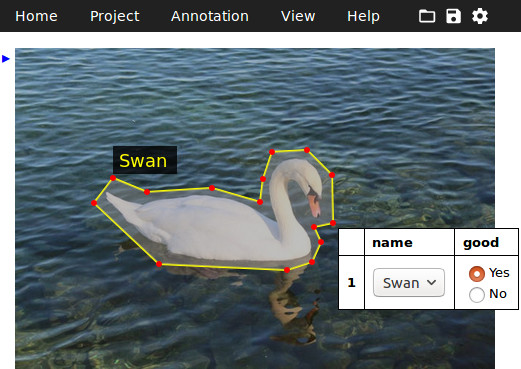
\includegraphics[width= 0.7\linewidth]{bab3/Demo Via.jpg}
		\caption{Software VIA \cite{dutta2019vgg}}
		\label{fig: VIA}
	  \end{center}
  \end{figure}
  
  \begin{figure}[h!]
	\begin{center}
	  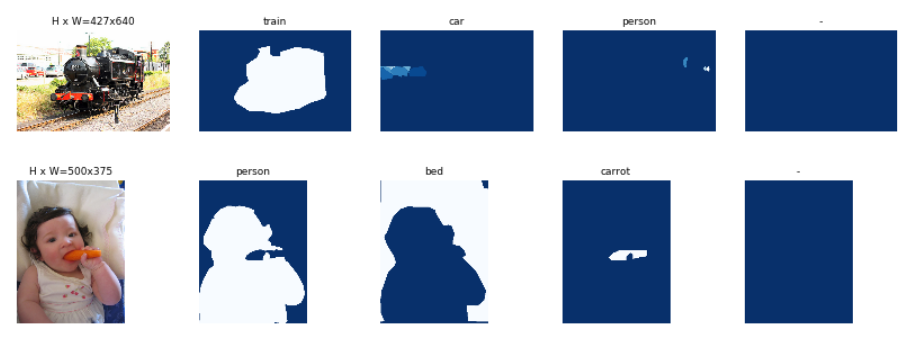
\includegraphics[width= 0.8\linewidth]{bab3/Contoh uji coba dataset.png}
	  \caption{Contoh Hasil Uji Coba Pembuatan Dataset \cite{matterport_maskrcnn_2017}}
	  \label{fig: Hasil Uji Coba}
	\end{center}
  \end{figure}
  
  
  \section{Data \textit{Preprocessing}}
  
  \begin{figure}[h!]
	  \begin{center}
		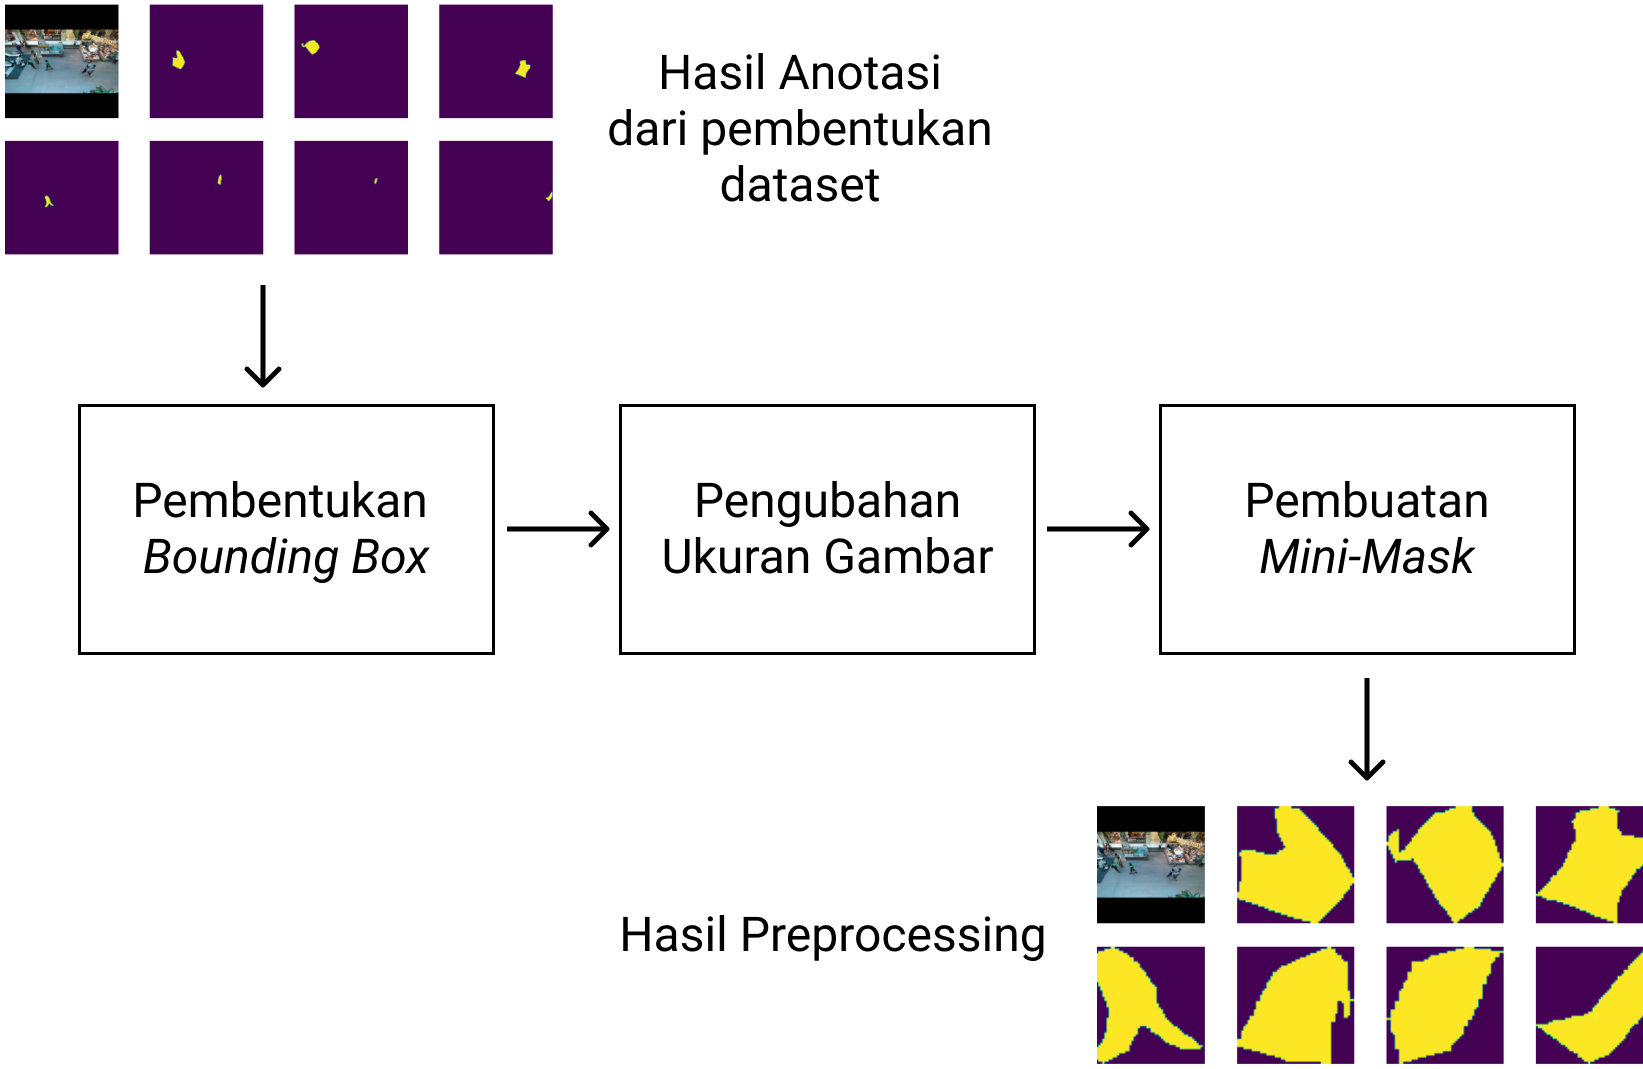
\includegraphics[width= 0.7\linewidth]{bab3/Preprocessing.png}
		\caption{Tahap \textit{Preprocessing}}
		\label{fig: Preprocessing}
	  \end{center}
  \end{figure}
  
  Pada tahap \textit{preprocessing} dataset yang telah dibentuk pada proses pembuatan dataset akan diolah terlebih 
  dahulu agar ukuran data menjadi lebih kecil dan
  proses ektraksi fitur maupun proses \textit{training} dapat dijalani secara lebih cepat dan tidak memerlukan 
  banyak sumber daya komputasi. Seperti yang telah tertera pada gambar \ref{fig: Preprocessing}, tahap \textit{preprocessing} dibagi menjadi 
  tiga yaitu pembuatan \textit{bounding box}, pengubahan ukuran gambar, dan pembuatan \textit{mini mask}.
  
  \subsection{Pembuatan \textit{Bounding Box}}
  Pada tahap ini,sbuah \textit{bounding box} akan dibentuk pada gambar-gambar yang telah memiliki objek anotasi.
  \textit{Bounding box} yang dibentuk mengikuti struktur panjang dan lebar segmentasi \textit{(mask)} yang telah 
  dibuat pada tahap pembuatan dataset. \textit{Bounding box} dibentuk mengikuti koordinat panjang dan lebar dari
  \textit{mask} agar jika gambar atau objek tersebut mengalami transformasi seperti pemutaran gambar, pengubahan
  ukuran gambar, dan pemotongan gambar, \textit{bounding box} dapat mengikuti koordinat transformasi dari 
  \textit{mask} pada objek yang telah melakukan transformasi. Proses ini tentunya lebih efektif daripada menghitung
  koordinat \textit{bounding box} setiap kali gambar melakukan transformasi.

  \subsection{Pengubahan Ukuran Gambar}
Pada tahap ini, setelah objek pada gambar diberikan \textit{bounding box} gambar akan diubah ukurannya menjadi
ukuran yang sama (\textit{uniform}) dimana pada penelitian ini, ditetapkan ukuran gambar adalah 1024 x 1024 karena
proses \textit{transfer learning} dari serta proses ekstraksi fitur mendukung ukuran tersebut. Jika gambar awal
tidak memiliki ukuran piksel 1024 pada kedua sisinya, maka sisi dengan nilai piksel terbesar akan diperpanjang 
hingga bernilai 1024, sedangkan sisi yang lain diperbesar mengikuti ratio awal. Jika salah satu sisi gambar telah
bernilai 1024, maka sisi yang lain akan ditambahkan piksel dengan nilai piksel 0 dimana gambar awal akhirnya
dipertahankan pada posisi tengah. Piksel bernilai 0 akan memberikan warna hitam pada gambar, sehingga pada proses 
ekstraksi fitur maupun deteksi citra, piksel bernilai 0 tidak memberikan dampak apapun dan hanya memakan sedikit 
daya komputasi.

\subsection{Pembentukan Mini Mask}
Pada tahap ini, setelah semua gambar memiliki nilai piksel yang sama, hasil segmentasi atau yang disebut
\textit{mask} pada data awal akan diekstrak dan mengalami perubahan ukuran. Pada awalnya \textit{mask} tiap objek
memiliki ukuran 1024 x 1024. Jika pada gambar tersebut memiliki banyak objek, misalnya sebagai contoh terdapat 10
objek, maka akan terdapat 11 gambar berukuran 1024 x 1024 piksel yang terdiri dari 10 gambar \textit{mask} dan 
1 gambar asli. Tentunya hal ini tidak efektif karena \textit{mask} tersebut akan memakan daya memori komputer 
saat melakukan proses \textit{training}, karena itu ukuran \textit{mask} akan diperkecil menjadi 56 x 56 piksel
dan hanya mengambil piksel \textit{mask}.

\section{Ekstraksi Fitur}

\begin{figure}[h!]
  \begin{center}
    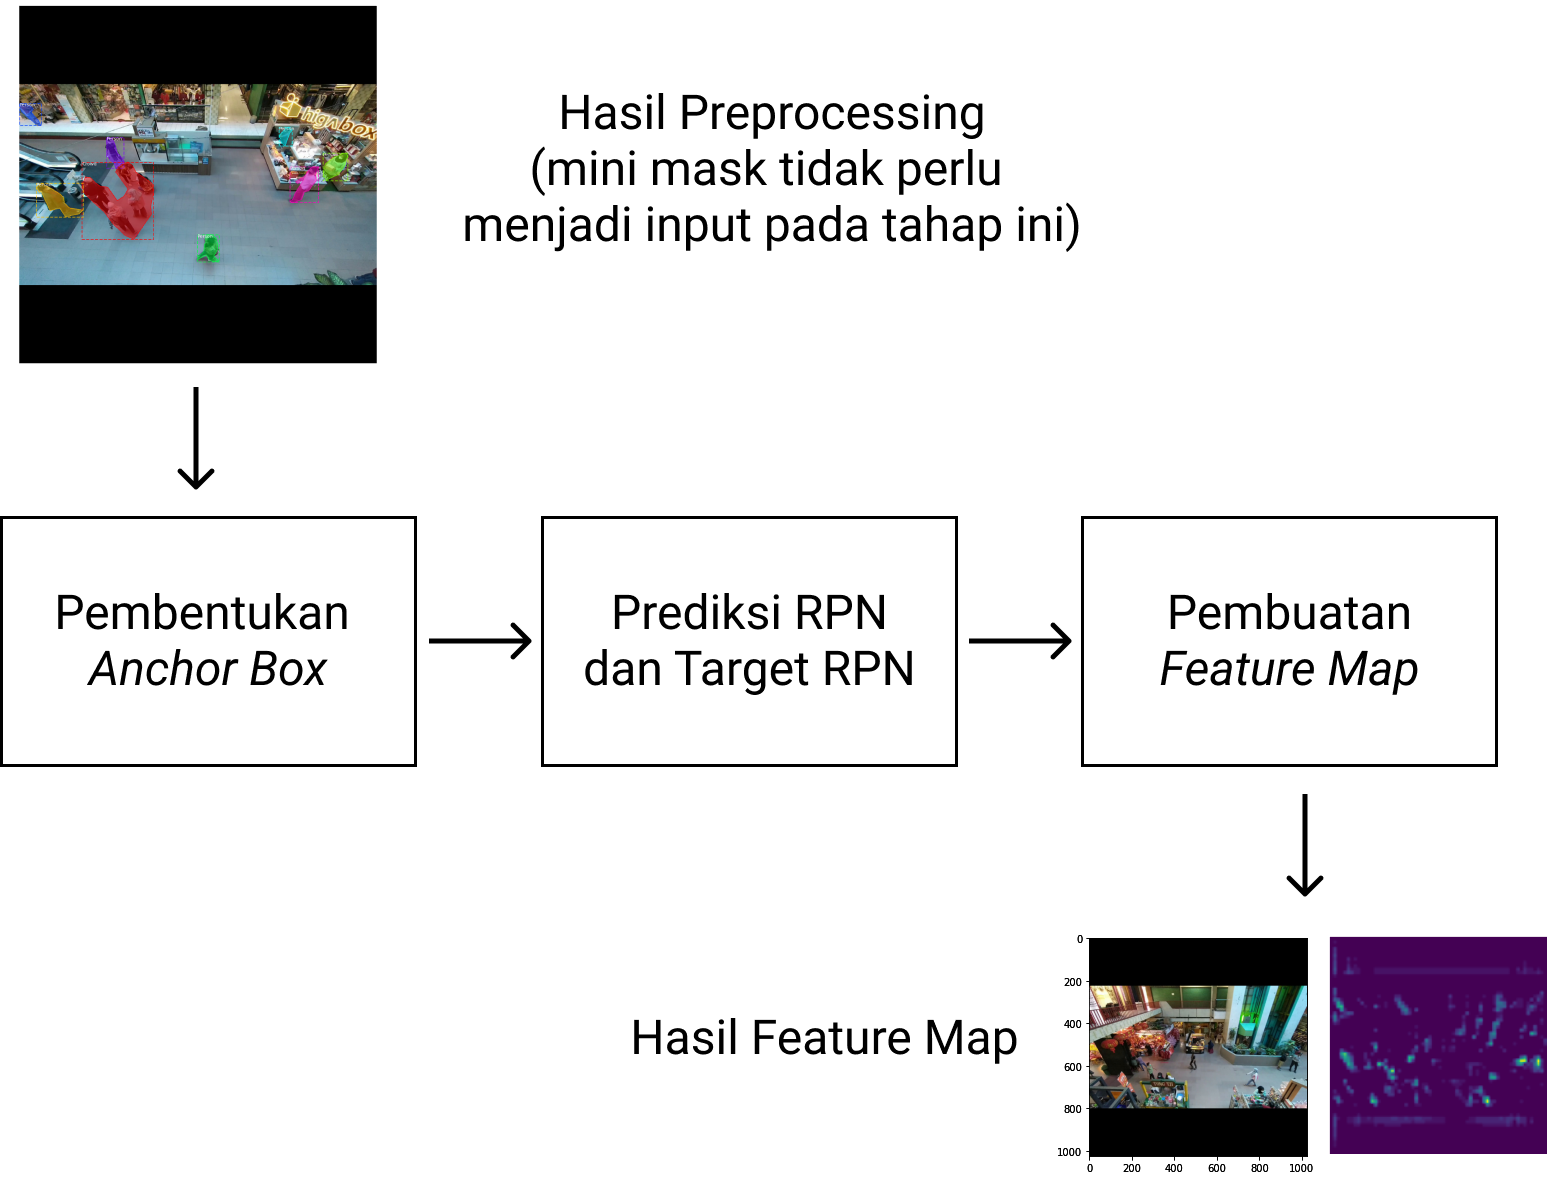
\includegraphics[width= 0.7\linewidth]{bab3/Ekstraksi Fitur.png}
    \caption{Proses Ektraksi Fitur}
    \label{fig: ekstraksi_fitur}
  \end{center}
\end{figure}

Proses ekstraksi fitur merupakan salah satu proses yang terpenting untuk memberikan data kepada algoritma deteksi
objek, dengan fitur-fitur yang diambil pada gambar, algoritma dapat menentukan lokasi serta kelas objek. Pada
penelitian ini, ekstraksi fitur menggunakan \textit{backbone} Resnet 101 yang memanfaatkan penggunaan 
\textit{anchor box}. Proses ekstraksi fitur yang perlu dilakukan pertama kali ialah membentuk \textit{anchor box},
kemudian berdasarkan \textit{anchor box} yang telah dibentuk, maka \textit{region proposal network} dapat dibangkitkan,
kemudian Resnet 101 akan digunakan untuk membuat sebuah \textit{feature map} berdasarkan \textit{region proposal
network} yang telah dibuat. \textit{Feature map} akan digunakan untuk mendeteksi lokasi, memberikan \textit{mask},
membangkitkan \textit{bounding box} dan mengklasifikasi kelas objek yang dideteksi.

\subsection{Pembuatan \textit{Anchor Box}}
Proses ekstraksi fitur yang pertama ialah pembuatan \textit{anchor box}, anchor box digunakan untuk mengetahui
lokasi \textit{bounding box} dan menjadi target dalam proses \textit{training} model dalam mendeteksi
\textit{regional proposal network (RPN)}. Terdapat 15 \textit{anchor box} yang dibentuk pada setiap iterasi.
Dapat dilihat pada gambar \ref{fig: Bentuk_Anchor_Box} bahwa \textit{anchor box} yang dibentuk memiliki lima
skala ukuran dan tiga jenis persegi empat yang mempunyai ukuran piksel yang berbeda. 15 belas \textit{anchor box}
tersebut akan disusun bertumpuk menyerupai piramid dan akan digeser setiap tiga piksel hingga semua piksel pada 
gambar telah terlingkupi oleh \textit{anchor box}. \textit{Anchor box} yang memiliki \textit{intersection over union}
atau irisan lebih dari sama dengan 70\% dengan \textit{bounding box} yang telah dibentuk pada tahap \textit{preprocessing}
dataset akan disimpan. Sedangkan \textit{anchor box} yang memiliki irisan kurang dari 70\% dengan \textit{bounding
box} yang telah dibuat akan dibuang dan tidak digunakan lagi. \textit{Anchor box} yang disimpan dinamakan 
target \textit{region proposal network} (RPN).

\begin{figure}[h!]
  \begin{center}
    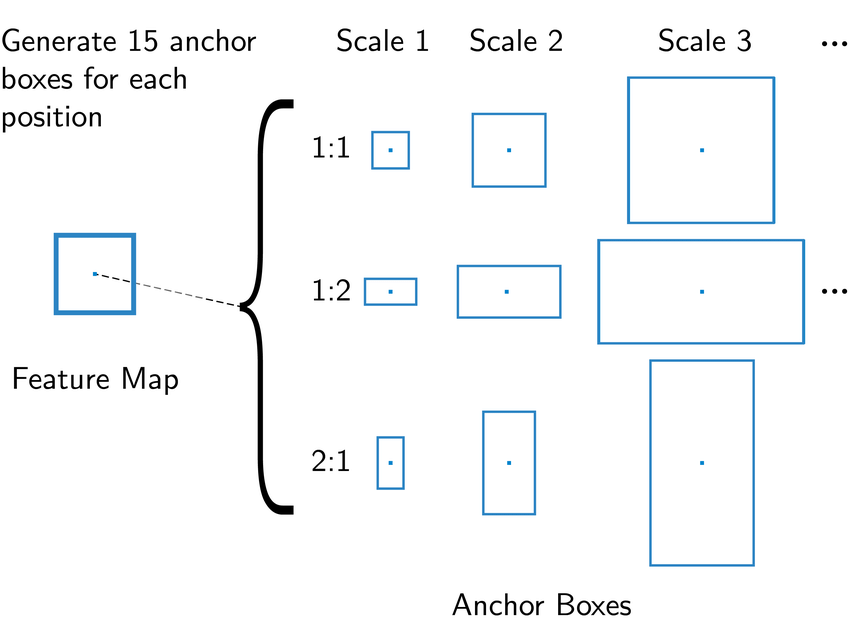
\includegraphics[width= 0.7\linewidth]{bab3/Anchor-Boxes-at-a-certain-position-in-the-feature-map.png}
    \caption{Bentuk \textit{Anchor Box} \cite{article_Anchor_Box}}
    \label{fig: Bentuk_Anchor_Box}
  \end{center}
\end{figure}

\subsection{Prediksi RPN}
Pada tahap sebelumnya, beberapa \textit{anchor box} yang mempunyai irisan dengan \textit{bounding box} asli telah
disimpan sebagai \textit{region of interest} positif . Target \textit{region proposal network} positif ini akan 
menjadi data untuk melatih model pada jaringan \textit{backbone}. Pada penelitian ini \textit{backbone} yang
digunakan ialah ResNet 101, sehingga jaringan \textit{Convolutional Neural Network} pada ResNet 101 akan dilatih
untuk dapat mendeteksi fitur yang ada pada \textit{regional proposal network}. Menggunakan beberapa iterasi maka
objek tersebut dapat dideteksi, kemudian suatu \textit{bounding box} hasil prediksi juga dibentuk, tentunya
\textit{bounding box} yang dibentuk terkadang dapat menimpa satu sama lain pada satu objek yang sama. Karena itu
penerapan algoritma \textit{non maximum supression} diperlukan agar \textit{bounding box} yang menimpa satu sama
lain dapat dihilangkan dan menjadi satu \textit{bounding box} yang optimal.

\subsection{Pembuatan \textit{Feature Map}}
Selain hasil berupa prediksi \textit{region proposal network}, \textit{backbone} ResNet 101 juga menghasilkan
sebuah \textit{feature map} yang merupakan hasil dari proses konvolusi dan pooling pada jaringan residual yang
digunakan. \textit{Feature map} ini akan digunakan sebagai data bagi \textit{fully connected layer} dan
\textit{layer konvolusi} untuk memprediksi kelas, \textit{bounding box}, dan \textit{mask}. Contoh hasil dari
\textit{feature map} dapat dilihat pada gambar \ref{fig: Feature Map example}.

\begin{figure}[h!]
  \begin{center}
    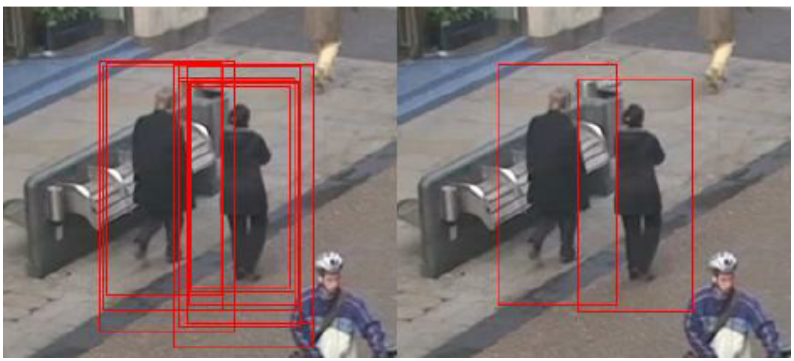
\includegraphics[width= 0.7\linewidth]{bab3/Non max suppression.png}
    \caption{Hasil \textit{non max supression} (kanan) \cite{Non_Max_Supression}}
    \label{fig: NMS}
  \end{center}
\end{figure}

\begin{figure}[h!]
  \begin{center}
    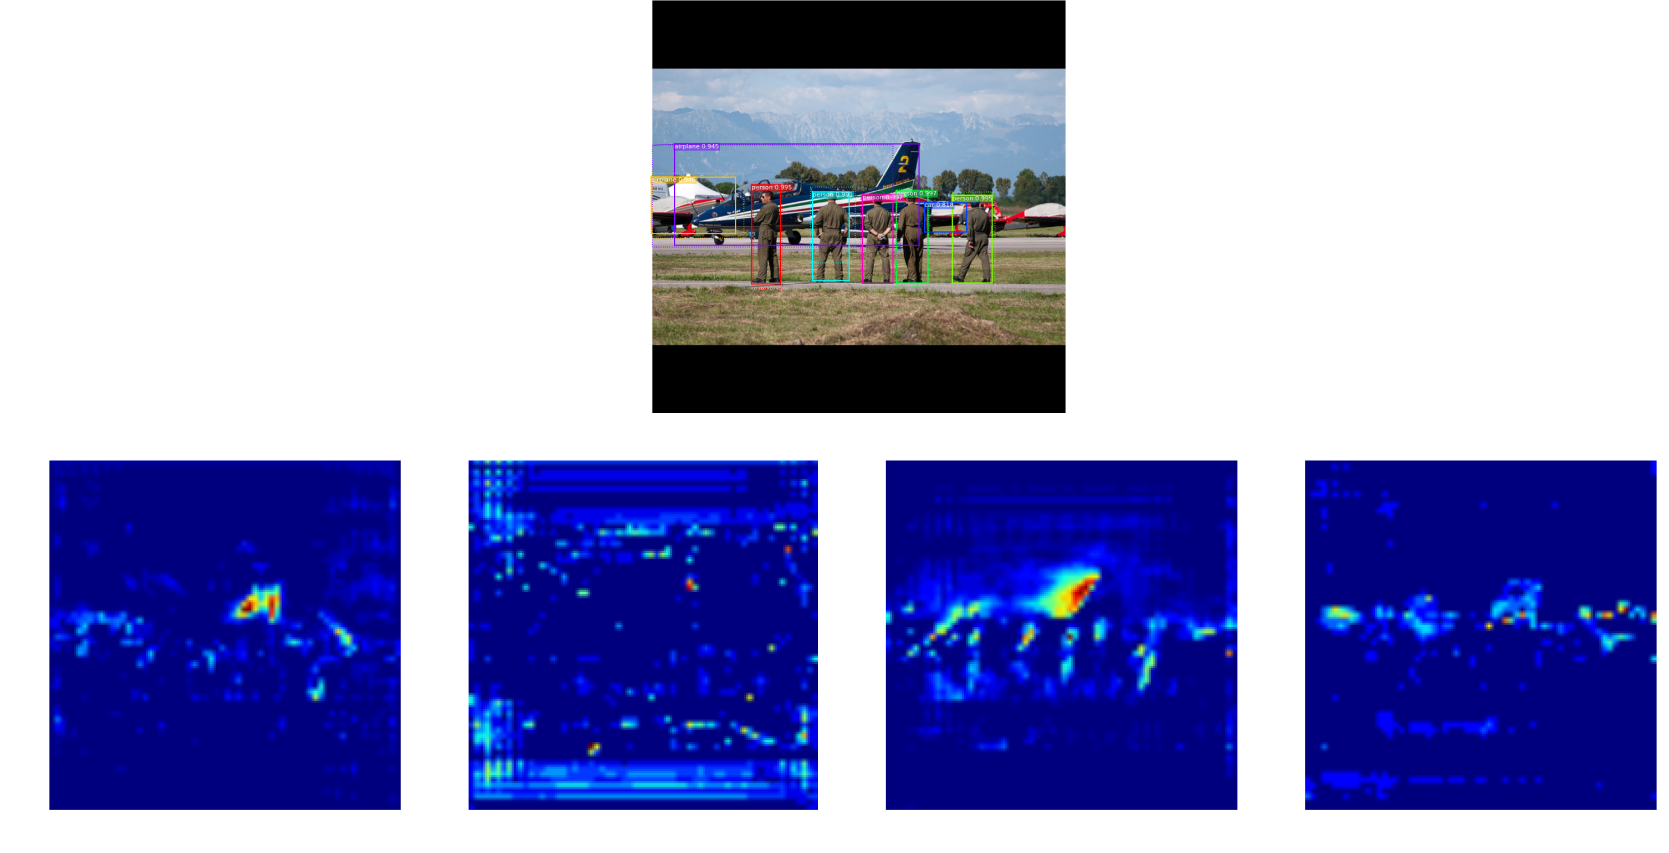
\includegraphics[width= 0.8\linewidth]{bab3/Contoh feature map.png}
    \caption{Contoh \textit{Feature map} pada \textit{layer} berbeda \cite{matterport_maskrcnn_2017}}
    \label{fig: Feature Map example}
  \end{center}
\end{figure}

\section{Proses Training}
Proses pembelajaran mesin sudah dilakukan pada tahap ekstraksi fitur, namun dalam mengklasifikasi
serta memberikan \textit{bounding box} yang tepat dari berbagai \textit{region proposal network} yang dibentuk
dari proses ekstraksi fitur, beberapa \textit{layer neural network} masih dibutuhkan dan perlu dilatih. 
Hasil keluaran dari \textit{layer convolutional neural network} dan \textit{fully connected layer} inilah yang
akan memberikan keluaran akhir dalam bentuk \textit{bounding box, mask}, dan kelas objek yang dideteksi.
Pada tahap ini sebuah \textit{fully connected layer} perlu dibentuk dalam mendeteksi kelas dan 
\textit{bounding box}. Selain itu, sebuah \textit{convolutional neural network} juga dibentuk untuk menghasilkan
\textit{mask} yang sesuai dengan objek. 

Pada tahap ini, beberapa \textit{hyperparameter} juga digunakan untuk mengatur
jalannya proses \textit{training}. \textit{Hyperparameter} yang daitur pada penelitian ini antara lain \textit{learning rate,epoch}
dan \textit{batch}. Pada penelitian ini pengaplikasian \textit{learning rate} dinamis juga akan diperkenalkan.
\textit{learning rate} dinamis digunakan dengan tujuan untuk mengurangi \textit{overfitting} dan mempercepat proses pembelajaran.
Pada \textit{epoch} 1 hingga 20, \textit{learning rate} yang digunakan adalah 0.01, pada \textit{epoch} 21 hingga
60, \textit{learning rate} yang digunakan adalah 0.005, sedangkan pada \textit{epoch} 61 hingga 150, 
\textit{learning rate} yang digunakan adalah 0.001 yang merupakan nilai terkecil yang digunakan pada penelitian
ini, detail \textit{learning rate} yang digunakan dapat dilihat pada tabel \ref{tab:lr_config}. Sedangkan
detail mengenai \textit{hyperparameter} dapat dilihat pada tabel \ref{tab:MaskRCCN_config}.

\begin{table}
  \caption{Konfigurasi pada proses \textit{training}}
  \label{tab:MaskRCCN_config}
  \centering
  \begin{tabular}{ | l | l | }
    \hline
    \textbf{Jenis Konfigurasi} & \textbf{Keterangan} \\ \hline
    \textit{batch}             & 1                   \\ \hline
    \textit{learning rates}    & dinamis dari 0.001 hingga 0.01                \\ \hline
    \textit{epoch}             & 150                   \\ \hline
  \end{tabular}
\end{table}

\begin{table}
  \caption{\textit{learning rate} dinamis}
  \label{tab:lr_config}
  \centering
  \begin{tabular}{ | l | l | }
    \hline
    \textbf{Epoch} & \textbf{Learning Rate} \\ \hline
    \textit{1 - 20}             & 0.01                   \\ \hline
    \textit{21 - 60}    & 0.005                \\ \hline
    \textit{61 - 150}             & 0.001                  \\ \hline
  \end{tabular}
\end{table}

\section{Proses Pengujian}
Proses pengujian model dalam penelitian ini dibagi menjadi 2 bagian, bagian yang pertama dilakukan pada saat 
model selesai melakukan proses \textit{training} namun masih memiliki iterasi \textit{epoch} yang belum selesai. 
Proses ini bernama validasi, dimana akurasi dari uji coba mode pada \textit{val set} akan dilakukan. 
Proses ini sangat vital karena dengan validasi kita dapat mengetahui apakah model 
kita mengalami \textit{overfitting} dimana performa model dalam mendeteksi objek di gambar baru dirasa kurang
maupun \textit{underfitting} dimana model tidak menunjukkan kemajuan dalam mendeteksi objek pada gambar. 
Salah satu ciri yang paling mudah yang 
menandakan kemungkinan terjadinya \textit{overfitting} adalah ketika besaran \textit{training loss} suatu model 
menjadi semakin kecil, namun besaran \textit{validation loss}-nya malah semakin besar di setiap iterasi. 
Sedangkan \textit{underfitting} terjadi ketika baik \textit{training loss} maupun \textit{validation loss} 
memiliki nilai yang terlalu besar. Selain itu pada proses validasi ini, data yang digunakan adalah data yang 
sama sekali baru dan tidak digunakan selama proses \textit{training} guna menghindari kemungkinan terjadinya 
bias yang biasa terjadi apabila suatu model diuji pada data yang sama yang digunakan pada saat proses 
\textit{training}. Berdasarkan data pada proses validasi, algoritma \textit{optimizer} akan memutuskan untuk 
merubah \textit{weight} dalam pada \textit{neural network} sehingga semakin mendekati titk akurasi tertingginya.

Bagian selanjutnya dari proses pengujian adalah melakukan \textit{test}. Sama seperti pada waktu proses validasi, 
dataset yang digunakan juga sama sekali berbeda dengan data yang digunakan pada waktu \textit{training} maupun 
pada waktu \textit{validasi}. Dari proses ini, dapat diambil kesimpulan apakah suatu model tersebut dapat 
dilakukan perbaikan lagi denga cara \textit{re-training} dan merubah beberapa parameter maupun konfigurasi 
yang sudah diatur pada saat proses \textit{training}, ataukah model tersebut dirasa sudah cukup baik dan akan 
melanjutkan ke proses berikutnya. Adapun beberapa metriks yang dapat diketahui dari proses 
\textit{training} yaitu metriks \textit{train accuracy, loss, val-accuracy} dan \textit{val-loss}.
\textit{loss function} yang diberikan merupakan jumlah segala \textit{loss} yang terjadi pada tiap tahapan
proses pada algoritma Mask R-CNN yang ditetapkan. Persamaan total \textit{loss} dapat dilihat pada persamaan
\ref{eq :loss}. Sedangkan persamaan total \textit{mask loss} dapat dilihat pada persamaan \ref{eq :mask loss}. Untuk
persamaan mengenai \textit{loss} yang terjadi pada kelas serta \textit{bounding box}, dapat dilihat pada
persamaan \ref{eq:other Loss}.

\begin{equation}
  \label{eq :loss}
  \mathcal{L} = \mathcal{L}_\text{cls} + \mathcal{L}_\text{box} + \mathcal{L}_\text{mask}
\end{equation}

\begin{equation}
  \label{eq:other Loss}
  \mathcal{L}_\text{fr} = \mathcal{L}_\text{cls} + \mathcal{L}_\text{box}
\end{equation}

\begin{equation}
  \mathcal{L}_\text{fr}(\{p_i\}, \{t_i\}) = \frac{1}{N_\text{cls}} \sum_i \mathcal{L}_\text{cls} (p_i, p^*_i) + \frac{\lambda}{N_\text{box}} \sum_i p^*_i \cdot L_1^\text{smooth}(t_i - t^*_i)
\end{equation}

\begin{equation}
  \label{eq :cls_loss}
  \mathcal{L}_\text{cls} (p_i, p^*_i) = - p^*_i \log p_i - (1 - p^*_i) \log (1 - p_i)
\end{equation}

\begin{equation}
  \label{eq :bbox loss}
  \mathcal{L}_\text{box} = \frac{\lambda}{N_\text{box}} \sum_i p^*_i \cdot L_1^\text{smooth}(t_i - t^*_i)
\end{equation}

\begin{equation}
  \label{eq :mask loss}
  \mathcal{L}_\text{mask} = - \frac{1}{m^2} \sum_{1 \leq i, j \leq m} \big[ y_{ij} \log \hat{y}^k_{ij} + (1-y_{ij}) \log (1- \hat{y}^k_{ij}) \big]
\end{equation}

\section{Analisa Performa}
Setelah melakukan proses pengujian, langkah berikutnya adalah melakukan analisa perforrma pada model yang 
sudah dibuat. Hal ini untuk mengetahui bagaimana kira - kira performa model pada saat sudah diimplementasi. 
Untuk analisa performa, model akan diuji pada dataset \textit{test}, dimana model tersebut akan mendeteksi
gambar-gambar yang belum pernah dilihat sebelumnya. Untuk mengetahui performa model, 
analisanya akan menggunakan beberapa metode seperti \textit{confusion matrix} untuk mendapatkan
pengelompokkan berdasarkan data menjadi \textit{True Positive} (TP), \textit{False Positive} (FP), 
\textit{True Negative} (TN), dan \textit{False Negative} (FN) dalam proses deteksi.
Selain itu, penelitian ini juga akan menggunakan rumus - rumus seperti \textit{Recall, Precision} dan 
\textit{Accuracy} dalam mengetahui performa model.






